\documentclass[twocolumn]{article}

%\usepackage[iso]{umlaute}
%\usepackage{german}
\usepackage{graphicx}
\setlength{\parindent}{0cm}
\setlength{\parskip}{1ex}
\setlength{\columnsep}{25pt}

\textwidth=17cm
\textheight=23cm
\setlength{\unitlength}{0.5cm}
\setlength{\parindent}{0.0cm}
\setlength{\parskip}{1ex}
\raggedbottom
\sloppy
%\addtolength{\evensidemargin}{-5cm}
\addtolength{\oddsidemargin}{-1.5cm}
\addtolength{\topmargin}{-2cm}

\sloppy

% Your name
\author{Trung Nguyen\\ Technische Universit\"at M\"unchen}

\title{Seminar Cloud Computing \\
       {\bf From Concept to Production: Enablements TinyML in Industrial Setting}
}

% Date of your talk
\date{November 2024}

\usepackage{hyperref}

\begin{document}

\maketitle

\begin{abstract}
In recent years, Artificial Intelligence (AI) and Machine Learning (ML) have received tremendous amount of attention in both industry and research world. However, conventional Machine Learning demands high computing capability which limits its usage to only larger computing units. The pardigm shift to Tiny Machine Learning (TinyML) is revolutionizing industries by enabling the deployment of machine learning models on low-power, resource-constrained devices. Being one of the most rapid developing field of Machine Learning, TinyML promises to benifits multiple industries. However, building a production-ready tinyML system poses different unique challenges. In this paper, we explore the key obstacles faced when developing and deploying TinyML models in production environments, including model optimization, hardware limitations, software integration, and maintaining performance in real-world conditions. Additionally, we present real-world use cases of TinyML in industrial settings, showcasing its transformative impact. We also discuss practical approaches and strategies presented by recent researches \cite{ren_tinyol_2021} to overcome these challenges, providing insights into how TinyML systems can be successfully scaled and implemented in production.
\end{abstract}

% \section defines numbered parts of the paper with titles
% there also are \subsection and \subsubsection
\section{Introduction}
\label{introduction}


Traditional Machine Learning Models, especially Deep Learning Models typically require substantial amount of computing capability to operate effectively. These models are often trained on powerful Graphics Processing Units (GPUs) and produce large models ranging from tens or hundreds of gigabytes (GB) down to smaller models in the range of 10 to 100 megabytes (MB). However, the memory requirements during runtime for these models far exceed what microcontrollers (MCUs) can handle.
The pardigm shift to TinyML is driven by the prevailing number of Microcontroller Units (MCU) currently circulating in the industry. According to a recent report \cite{noauthor_microcontroller_nodate,grandviewresearch_research_2023}, as of 2021, around 31 billion MCUs were shipped worldwide annually. The MCU market size is projected to increase in upcoming years \cite{noauthor_microcontroller_nodate}. This creates a big incentive for researchers and industry players to put effort into developing the technology further.
TinyML aims to enable data processing or inferencing directly on embedded systems, particularly on Internet Of Things (IOT), instead of streaming to the cloud. TinyML model can run on energy-, and memory-constraint devices by limiting communication overhead with better suited architecture design and applying different compressing techniques such as: quantization and pruning. The advancement of tinyML has positively influenced multiple industries/sectors such as: industrial IOT \cite{ray_review_2022}, healthcare \cite{bhamare_chapter_2024}, agriculture \cite{tsoukas_tinyml-based_2022}, IOT in smart-city \cite{hussein_original_2024,ray_review_2022}. \\[0.25cm]

Although various organizations have been actively investing resources into machine learning projects, only around 13\% of these projects successfully progress to production. This low success rate highlights the complex challenges and gaps in translating ML concepts into fully functional, production-grade systems, especially in the realm of TinyML. In this paper, we aim to address these challenges and outline what is necessary to transition a TinyML project from concept to production, ultimately creating value for industrial applications. In Chapter~\ref{tinyml_overview}, we provide an in-depth overview of the fundamental concepts, techniques, and development pipeline of TinyML. Following this, in Chapter~\ref{prod_tinyml}, we draw on recent research to investigate the specific challenges encountered in developing and deploying TinyML models in production environments, as well as practical strategies to overcome these obstacles. Next, in Chapter~\ref{use_cases}, we explore real-world applications of TinyML in industrial settings, illustrating its transformative potential. Finally, in Chapter~\ref{future_of_tinyml}, we consider the future trajectory of TinyML, discussing upcoming advancements and their implications for broader industrial adoption.
\begin{figure}
	\centerline{
	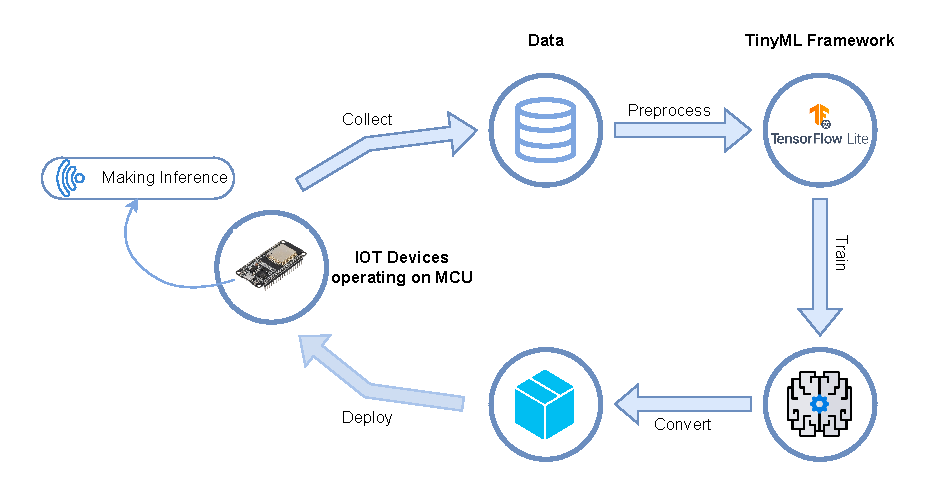
\includegraphics[width=1\columnwidth]{resource/tinyml_deployment.pdf}
	}
	\caption{The caption explaining what can be seen in the image/figure.
	Readers often read captions first if they do not have much time. Thus,
	it is important to find a good short explanation.}
	% A label to allow refering to this figure in the text.
	\label{TUM}
\end{figure}

\section{TinyML Overview} 
\label{tinyml_overview}

\subsection{Key Concepts and Techniques}

Pruning removes unnecessary neurons or connections from a neural network to reduce its size and complexity. This optimization lowers memory and computational demands, making the model faster and more efficient for deployment on resource-limited devices like microcontrollers.

Quantization reduces the precision of model parameters (e.g., from 32-bit to 8-bit), which decreases model size and computational needs. This technique enables efficient model inference on devices with limited memory and processing power, such as those used in TinyML applications.

With the TinyML model running on edge, the data is stored, processed and analysed internally rather
than at an external server or cloud. 

\subsection{TinyML pipeline}

Data Collection:
	•	The workflow starts with collecting data from an IoT device. This data serves as the input for training machine learning models. The IoT device can gather various types of data depending on the application, such as sensor data in smart homes or environmental monitoring. \\[0.25cm]
Preprocessing:
	•	After collecting data, it moves to the preprocessing stage. Here, the data is cleaned and prepared for model training. Preprocessing can involve tasks such as normalization, handling missing values, or feature extraction to improve the quality of the input data.\\[0.25cm]
Model Training:
	•	The preprocessed data is fed into an ML framework, where a machine learning model is trained. This stage involves using machine learning algorithms to find patterns in the data, building a predictive or analytical model that can generalize from the data.\\[0.25cm]
Model Conversion:
	•	Once the model is trained, it is converted into a format suitable for deployment on resource-constrained devices, like microcontrollers. This step might involve techniques such as quantization (reducing the precision of model weights) or pruning (removing unnecessary parts of the model) to reduce the model’s size and computation needs.\\[0.25cm]
Model Packaging:
	•	After conversion, the model is packaged into a deployable form. This includes bundling the model with any necessary runtime components to allow it to be executed efficiently on the target device.\\[0.25cm]
Deployment:
	•	The next step involves deploying the packaged model onto an IoT device. This means transferring the model to the device, setting it up for real-time inference or operation in the field.\\[0.25cm]
Inference:
	•	Finally, the deployed model performs inference on the IoT device. Inference refers to the process of using the model to make predictions or decisions based on new data collected by the IoT device. The model operates locally on the device without needing continuous cloud connectivity, enabling real-time decision-making at the edge.\\[0.25cm]



\section{Enablements of TinyML in Industrial Setting}
\label{prod_tinyml}

\subsection{Challenges}

The fundamental pipeline for deploying a TinyML model to a microcontroller, as described above, provides a general framework for model development and deployment. However, in industrial settings, this pipeline often falls short due to a variety of challenges unique to production environments.


\subsubsection{Performance across heterogeneous devices or affected by heterogeneity}
\subsubsection{Adaptation to unseen scenarios and constantly changing conditions
}

\subsubsection{Model and device management at scale}


% use \cite to refer to papers from seminarpaper.bib
% this file is processed by bibtex, and it automatically adds numbering
\cite{hussein_original_2024, paul_rethinking_2021, de_prado_robustifying_2020,ren_synergy_2021,roshan_adaptive_2021}.


\subsection{Bringing tinyML to production environment}


\section{Use Cases of TinyML in Industrial Setting}
\label{use_cases}

Enumerations using bullet points:

\begin{itemize}
	\item 	Agriculture
	\item 	Environmental Monitoring
	\item 	Industrial predictive maintenance
	\item 	Edge AI and Autonomous Systems
\end{itemize}


\section{Future of TinyML }
\label{future_of_tinyml}



\section{Conclusion}
\label{conclusion}



% Put citations from bibtex into References section which were not
% explicity cited.
\nocite{hussein_original_2024,paul_rethinking_2021}


\bibliographystyle{plain}
% Literature sources are to be found in seminarpaper.bib
\bibliography{seminarpaper}
\end{document}
